

\chapter{Absence of Information is also Knowledge}

This chapter presents an alternative approach to the problem of learning object placement habits of humans in an occluded environment. We assume there is a domestic service robot which while interacting in human environments records all the information generated using its vision sensor.
Generally in domestic environments like our home, we humans prefer to store our food, cooking equipment, silverware and dishes inside closed cabinets like drawers, cupboards and refrigerators. So most of the time the objects are inside cabinets which cannot be observed using a vision sensor. For a domestic robot with only camera as a sensor, the chances of observing  these objects inside closed cabinets is drastically reduced.
\missingfigure{Occluded kitchen with labelled location names and bounding box object name}
The basic requirement of machine learning is data, from which information and knowledge can be learnt. But in highly occluded environments like kitchen its difficult for a domestic robot to make an observation of the object and record the object location.  Hence our hypothesis that we can learn knowledge about object locations quantitatively i.e. learning patterns from the data observed, becomes a herculean task to prove.

An alternative approach to counter the sparsity of data is by recording the absence of the object in visible locations and learning knowledge about where objects are not located. Consider an motivating example, as depicted in Figure \cite{fig:alllocations} . Here, a mobile robot is in a kitchen in the morning. The following locations can be scanned by the robot: kitchen-sink, counter-top and stove, while the cabinets, dishwasher and refrigerator are occluded. The robot will make observations of cup and kettle on counter-top , spoon on the sink top. Assume that the robot is also learning object locations of cooking pot. If the robot only records the observed objects then there is no data recorded for the cooking-pot and no knowledge is learned about the cooking-pot. \emph{A possible solution is to even record the \textbf{absence} of cooking-pot on the visible locations}. From this the robot can learn that the cooking-pot is less probable to be on the kitchen-sink, counter-top and stove during morning time. Supplementary the robot can also learn that there is higher probability for the cooking-pot being in the cabinet or dishwasher.

\section{Simulated Dataset: Kitchen Object Dataset}

To demonstrate the proposed approach we have generated a kitchen object dataset. The dataset consist observations(presence and absence) of a cup in a kitchen environment made by a domestic robot. The robot can scan 4 locations in the kitchen: sink, counter-top, stove and cabinet. The time of the scan is discretized into 3 times of the day: morning, afternoon and night. 

\begin{figure}
    \centering
    \begin{subfigure}[b]{0.3\textwidth}
        \includegraphics[width=\textwidth]{images/sink.jpg}
        \caption{Sink}
        \label{fig:sink}
    \end{subfigure}
    ~ %add desired spacing between images, e. g. ~, \quad, \qquad, \hfill etc. 
      %(or a blank line to force the subfigure onto a new line)
    \begin{subfigure}[b]{0.3\textwidth}
        \includegraphics[width=\textwidth]{images/stove.jpg}
        \caption{Stove}
        \label{fig:stove}
    \end{subfigure}
    ~ %add desired spacing between images, e. g. ~, \quad, \qquad, \hfill etc. 
    %(or a blank line to force the subfigure onto a new line)
    \begin{subfigure}[b]{0.3\textwidth}
        \includegraphics[width=\textwidth]{images/counter-top.jpg}
        \caption{counter-top}
        \label{fig:counter-top}
    \end{subfigure}
    \caption{Different possible object locations}\label{fig:alllocations}
\end{figure}

The generative process for each possible observation(present and absent) in the dataset 
\begin{itemize}
    \item Choose $ \theta \sim Dirichlet(\alpha)$ (Distribution of object over location-time)
    \item Choose randomly the time period $i$.
	\item Choose the location $x_n$ $\sim$ Categorical$(\theta_i)$
	\item Choose the presence of object $p_n$, in time period $i$ and location $x_n$  $p_n$ $\sim$ Bernoulli$(\beta) $
\end{itemize}

Ground truth of the distribution in the object location distribution over time in shown in Figure \todo{cite image}.


\begin{figure}[htp]
\centering
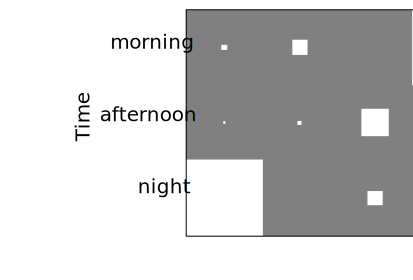
\includegraphics[width=0.6\textwidth]{images/absent_groundtruth.png}
\caption{Simulated object location ground truth distribution}
\medskip
\small
The x-axis represents the locations the y axis represents the timezones. The size of the white box indicates the probability of the object presence.
\label{absent-gt}
\end{figure}

From the ground truth we can observe that there is higher probability to find the object in the sink during night time and in the cabinet during the other time periods. We need to develop models which can learn these temporal patterns from the observations


\section{Dirichlet-Categorical-Bernoulli model}

For incorporating the negative instances we modified the Dirichlet-Categorical model explained in section \todo{cite chapter} with a Bernoulli model. But Bernoulli 


\begin{minipage}{0.3\textwidth}
\centering

\tikz {
\node [const]                   (alpha) {$\alpha$};
\node [below=of alpha, latent]  (beta)  {$\beta$};
\node [below=of beta, latent]   (theta) {$\theta_i$};
\node [below=of theta, obs]     (x)     {$x_{ij}$};
\node [above=of x , xshift=1.8cm, latent]      (gamma) {$\gamma$};
\edge {alpha} {beta};
\edge {beta} {theta};
\edge {theta} {x};
\edge {gamma} {x};
\plate {trials} {(x)} {j location};
\plate {bags} {(theta)(x)(trials)} {i time};
}

\end{minipage}%
\begin{minipage}{0.7\textwidth}

\begin{equation*}
	\alpha = <1, 1, .... , 1 > 
\end{equation*}
\begin{equation*}
	\beta \sim Dirichlet(\alpha)
\end{equation*}
\begin{equation*}
	\theta_i  \sim Dirichlet(\beta)
\end{equation*}
\begin{equation*}
	\gamma  \sim Bernoulli(k)
\end{equation*}

\begin{equation*}
	x_{ij} \sim Categorical(\theta_i)
\end{equation*}
\end{minipage}

\section{Evaluation}

The proposed models are evaluated on the simulated dataset. We compare the Dirichlet-Categorical-Bernoulli model with the Hierarchical-Dirichlet-Categorical model explained in \todo{cite }. We compare the dirichlet probability used to generate the simulated dataset and the learned probabilities and evaluate the performance of the learning. 
We use the adopted  Bhattacharyya distance \todo{cite } to quantify the similarity between the simulated and the learned distribution.

 The Bhattacharyya distance is a measure of divergence between
probability distributions, that allows measuring the dissimilarity between two continuous or discrete probability distributions. It can take values from 0-$\inf$. The value is 0 when both the distributions are similar and $\inf$ when there is no overlap between the distributions. Adopting the  Bhattacharya distance to Dirichlet distributions [Rauber et al ]\todo{cite Rauber} we get :
\begin{multline}
	D_B(Dir_a(x_1, \dots ,x+n), Dir(y_1, \dots , y_n)) = \nonumber\\
	 \Gamma \Bigg( \frac{1}{2}  \sum_{i \in {1, \dots, n}} x_i +  \frac{1}{2}\sum_{i \in {1, \dots, n}} y_i\Bigg) + 
	\frac{1}{2}  \sum_{i \in {1, \dots, n}} \Gamma (x_i) + 
	\frac{1}{2}  \sum_{i \in {1, \dots, n}} \Gamma (y_i) - \\ 
	\sum_{i \in {1, \dots, n}} \Gamma \bigg(\frac{1}{2} (x_i + y_i) \bigg) - \frac{1}{2}  \Gamma \Bigg(  \sum_{i \in {1, \dots, n}} x_i \Bigg) + \frac{1}{2}  \Gamma \Bigg( \sum_{i \in {1, \dots, n}} y_i\Bigg)
\end{multline}

The distance

\section{ss}


A . Bhattacharyya.  On  a  measure  of  divergence  between two  statistical populations  defined  by  their  probability distributions.    Bull.  Calcutta Math.  Soc.,  49:214–224, 1943

T.W. Rauber, A. Conci, T. Braun, and K. Berns. Bhattacharyya probabilistic distance of the dirichlet density and its application to split-and-merge image seg- mentation. In WSSIP08 , pages 145–148, 2008. 

